%% Do not edit unless you really know what you are doing.
\documentclass[french,english,12pt]{exam}

%\printanswers

\usepackage{tikz}

\usepackage{../../latex/macro_mealor}
\usepackage{../../latex/structuralanalysis}
\usepackage[utf8]{inputenc}
\usepackage[T1]{fontenc} % accents codés dans la fonte
%\usepackage{layout}
\usepackage{a4wide}
%\usepackage[french]{babel}
\usepackage{hyperref}

\usepackage{graphicx}
\usepackage{caption}

\usepackage{newpxtext,newpxmath}
\usepackage{siunitx}

%\setlength{\hoffset}{0pt}
%\setlength{\oddsidemargin}{-1cm}   % Marge gauche sur pages impaires
%\setlength{\evensidemargin}{-1cm}   % Marge gauche sur pages paires
%\setlength{\marginparwidth}{0cm}   % Largeur de note dans la marge
%\setlength{\textwidth}{16cm}   % Largeur de la zone de texte (17cm)
\setlength{\voffset}{0pt}   % Bon pour DOS
\setlength{\marginparsep}{0pt}   % Séparation de la marge
\setlength{\topmargin}{0cm}   % Pas de marge en haut
\setlength{\headheight}{0cm}   % Haut de page
\setlength{\headsep}{0cm}   % Entre le haut de page et le texte
%\setlength{\footskip}{1cm}   % Bas de page + séparation
%\setlength{\textheight}{25.5cm}   % Hauteur de la zone de texte (25cm)

\usepackage{indentfirst}


\newcommand{\classurl}{\url{1}}
% #1 numéro de la feuille
% #2 titre de la feuille
\newcommand{\titre}[3] {%\textit{
  \begin{center}\textbf{\textsc{MEALOR II}}\\ \textit{Mécanique de l'endommagement et approche locale de la rupture}%\let\thefootnote\relax\footnotetext{\classurl} 
  \end{center}
 
  \noindent TD n\textdegree #1 \hfill  August 2023\\[-0.3cm]
  \rule{\linewidth}{.3mm}
  \vspace*{0.5pt}
  \begin{center}
    {
      \Large \bfseries { #2}
    }\\
    \vspace*{0.5cm}
	\large #3
    \vspace*{0.5cm}
  \end{center}
}

\usepackage{xcolor}
\definecolor{Blue}{RGB}{0,68,170}
\SolutionEmphasis{\normalfont\color{Blue}}
\DeclareCaptionFont{blue}{\color{Blue}}

\newenvironment{objectifs}
    {\itshape\underline{Objectifs:}\begin{itemize}
    }
    { \itshape
    \end{itemize}
    }
    
\newcounter{Rfig}
\newenvironment{R_figure}
   {\begin{minipage}{\linewidth}\begin{center}\vspace{0.5mm}\stepcounter{Rfig}\addtocounter{figure}{-1}\renewcommand\thefigure{R-\arabic{Rfig}}
   \captionsetup{font=blue}}
   {\end{center}\vspace{0.5mm}\end{minipage}}
   
    
\newcounter{Rtab}
\newenvironment{R_table}
   {\begin{minipage}{\linewidth}\begin{center}\vspace{0.5mm}\stepcounter{Rtab}\addtocounter{table}{-1}\renewcommand\thetable{R-\arabic{Rtab}}
   \captionsetup{font=blue}
}
   {\end{center}\vspace{0.5mm}\end{minipage}}
   
      
\graphicspath{{./pic/}}
\usepackage{subcaption}

\newcommand{\jb}[1]{{\textcolor{red}{#1}}}

\begin{document}
\thispagestyle{empty}
\titre{4}{Les modèles variationnels de rupture en 1d: barre en traction}{Jérémy Bleyer, Corrado Maurini}
%\maketitle
\begin{objectifs}
\item Manipuler les conditions d'optimalité d'une fonctionnelle et appliquer l'approche variationnelle à la rupture dans le cas 1d
\item Déterminer l'évolution quasi-statique d'un modèle d'endommagement
\item Comprendre l'origine des contraintes limites et de la ténacité dans les modèles d'endommagement à gradient.
\item Assimiler les bases des modèles de rupture de type champs de phase avant la mise en \oe{}uvre numérique.
\item Construire des solutions de référence pour la vérification d'un code numérique de type champs de phase.
\end{objectifs}

\section*{Contexte}
Les modèles variationnels de rupture sont à la base des approches de type champs de phase pour la simulation numérique des phénomènes de rupture fragile. 
Dans cet exercice, on se propose de retrouver les propriétés fondamentales de ces modèles dans le cadre simplifié d'une barre en traction. 


\begin{figure}[h!]
\begin{center}
    \begin{tikzpicture}
    \point{a}{0}{0};
    \point{b}{6}{0};
    \point{e}{6.1}{0};
    \point{d}{7.5}{0};
    \point{c}{3}{0};
    \support{3}{a}[-90];
    %\support{3}{b}[90];
    \beam{2}{a}{b}[0][1];
%    \dimensioning{3}{e}{d}{-1.}[$u(L)=t\,L$];
    %\dimensioning{1}{e}{d}{1}[$u(L)=t\,L];
    \notation{1}{e}{$u(L)=t\,L$}[above];
    \load{1}{d}[180]
   % \dimensioning{3}{a}{b}{.5}[$\Delta s$];
    %\dimensioning{2}{a}{b}{-1.}[$L$] ;
    \dimensioning{1}{a}{b}{-1.}[$L$] ;
    %\notation{3}{a}{b}[$i$];
    %\temperature{a}{b}{-.5}{.5};
    \end{tikzpicture}
\end{center}
    \caption{Barre en traction avec déplacement imposé à l'extrémité.}\label{fig:barre}
\end{figure}
On considère une barre encastrée en $x=0$ et avec un déplacement imposé $u(L)=t\,L$ en
$x=L$.  On note par $E_0$ le module de Young du matériau
constituant la barre (dans son état non endommagé), $G_c$ sa
ténacité, $S$ la
surface de la section droite et $L$ la longueur. Dans la suite, on étudie le
problème de rupture de la barre avec un modèle de Griffith et un modèle
d'endommagement à gradient.

\section{Solution élastique : approche variationnelle}
On suppose ici que la barre est élastique linéaire. On se propose de déterminer la solution de ce problème simple avec l'approche variationnelle de l'élasticité.

L'énergie potentielle élastique de la barre est 
\begin{equation}
	\mathcal P(u)=\int_\Omega \frac{E_0S}{2}\left(
	\frac{du}{dx}
		(x)\right)^2 dx
	\label{eq:energie-elastique}
\end{equation}
où $u:x\in\Omega\equiv[0,L]\to u(x)\in\mathcal R$ désigne  le déplacement axial de la
barre.
Le problème de recherche de configurations d'équilibre peut être formulé comme un problème de minimisation de l'énergie potentielle. La configuration d'équilibre $u$ doit être celle qui minimise l'énergie parmi toutes les configurations admissibles $\hat u \in\mathcal{C}_t$, où $\mathcal{C}_t$ est l'espace des configurations admissibles :
\begin{equation}
u\in\mathcal{C}_t: \,\mathcal{P}(u+h(\hat u-u))-\mathcal
{P}(u)\geq 0,\forall \hat u\in\mathcal C_t.
\label{eq:energy-variation}
\end{equation}
L'espace des configuration admissibles est donné par les fonctions qui respectent les conditions aux limites de Dirichlet et qui sont assez régulières pour que $\mathcal{P}(u)\leq +\infty$:
\begin{questions}
    \question 
    Donner l'expression de $\mathcal{C}_t$ pour la barre de figure~\ref{fig:barre} et montrer, avec un développement limité en $h$ de la variation de l'énergie~\eqref{eq:energy-variation}, qu'une configuration d'équilibre doit satisfaire la condition suivante, formulation faible du problème d'élasticité :
    \begin{equation}
        D_u\mathcal{P}(u)(v)=0,\quad \forall v\in \mathcal{C}_0
        \label{eq:elasticite-foc}
    \end{equation}
    où on note 
    $$
    D_u\mathcal{P}(u)(v):=\left.\dfrac{d}{dh}\mathcal{P}(u+hv)\right\vert_{h=0}
    $$
    et donner pour notre exemple l'expression de 
    $\mathcal{C}_0$, défini comme l'espace vectoriel des variations admissibles, constituées par les différences entre fonctions admissibles.
    \begin{solution}
        Les fonctions admissibles doivent avoir des dérivées premières à carré intégrables dans $\Omega$, pour avoir une énergie finie et respecter les conditions aux limites :
        $$\mathcal{C}_t=\{u\in H^1(0,L),\,u(0)=0,\,u(L)=t\,L\}
        $$
        Soit $v=\hat u-u\in\mathcal{C}_0$. Le développement en $h$ de la condition de minimalité donne
        $$
        0\leq\mathcal{P}(u+h\,v)-\mathcal{P}(u)=h\left.\frac{d}{dh}\mathcal{P}(u+h\,v)\right\vert_{h=0}+o(h).
        $$
        donc au premier ordre on doit avoir:
        $$D_u\mathcal{P}(u)(v)\geq 0$$
        $\mathcal{C}_0$ étant un espace vectoriel, $\forall v\in\mathcal{C}_0$,  $-v\in \mathcal{C}_0$. Par la linéarité de la dérivée, 
        $D_u\mathcal{P}(u)(-v)=-D_u\mathcal{P}(u)(v)$. Donc on doit avoir $D_u\mathcal{P}(u)(v)= 0$.
        
    \end{solution}
    \question Calculer $D_u\mathcal{P}(u)(v)$ et montrer que la condition~\eqref{eq:elasticite-foc} implique la condition d'équilibre
    \begin{equation}
        \frac{d}{dx}\sigma(x)=0,\quad \text{avec}\quad\sigma=E_0S\frac{d u}{dx}(x).
        \label{eq:equilibre}
    \end{equation}
    \begin{solution}
        $$D_u\mathcal{P}(u)(v)=
        \left.\frac{d}{dh}
        \int_0^L\frac{E_0S}{2}(u'(x)+h\,v'(x))^2\,\mathrm{d}x\,\right\vert_{h=0}
        =\int_0^L \underbrace{E_0S u'(x)}_{\sigma}v'(x)\mathrm{d}x
        $$
        Après intégration par partie en utilisant que $v(0)=v(L)=0$:
        $$
        \int_0^L -\sigma \,v(x)\mathrm{d}x=0,\quad\forall v\in\mathcal{C}_0
        $$
        $v$ étant arbitraire, le lemme fondamental du calcul des variations impose donc que :
        $$
        \sigma'(x)=0,\quad\forall x\in(0,L)
        $$
    \end{solution}
    \question Déterminer les champs de déplacement $u_t$ et contrainte $\sigma_t$ solution du problème.  Montrer que l'énergie potentielle à l'équilibre en fonction du chargement est :
    \begin{equation}
        \mathcal{P}(u_t)=\min_{u\in\mathcal{C}_t}\mathcal{P}(u)=E_0S\,L\,\frac{t^2}{2}
        \label{eq:energie-elastique-sol}
    \end{equation} 
    \begin{solution}
        L'équation d'équilibre donne :
    $$
    E_0S\left(\frac{du_t}{dx}(x)\right)=\sigma_t\Rightarrow \frac{du_t}{dx}(x)=\frac{\sigma_t}{E_0S}\Rightarrow u_t =\left(\frac{\sigma_t}{E_0S}\right)x+u(0)
    $$
    En utilisant les conditions aux limites $u\in\mathcal C_t\rightarrow u(0)=0,u(L)=t\,L$ on trouve l'unique solution
    $$
    u_t=t x,\quad \sigma_t=E_0S\,t
    $$
    En remplaçant dans l'énergie potentielle~\eqref{eq:energie-elastique} on trouve~\eqref{eq:energie-elastique-sol}.
    \end{solution}
\end{questions}

\section{Modèle de Griffith}
Dans un modèle de type "interphase franche" de rupture à la Griffith, les fissures forment un ensemble de points $\Gamma\equiv\{\bar x_i\}_{i=1}^n$ où les déplacements peuvent être discontinus.  
On considère ici pour la barre un modèle de Griffith monodimensionnel,
caractérisé par l'énergie totale
\begin{equation}
	\quad \mathcal{E}_G(u,n)=\int_{\Omega\setminus\Gamma} E_0S\left(
	\frac{du}{dx}
		(x)\right)^2 dx + G_c\,S \,n
	\label{minprob}
\end{equation}
où $u:x\in[0,L]\to u(x)\in\mathcal R$ représente  le déplacement axial de la
barre et $n$ le nombre des fissures. 
L'approche variationnelle de la rupture (Francfort-Marigo 1998) définit la solution du problème comme le minimum global de l'énergie $\mathcal{E}_G(u,n)$, sous une contrainte d'irréversibilité pour les fissures.


\begin{questions}
\question En utilisant les résultats de la section précédente, calculer $\mathcal{E}_G(u,0)$ et $\mathcal{E}_G(u,1)$ en fonction de $t$. Calculer le chargement critique $t_G$ pour la fissuration de la barre selon ce modèle. Discuter de la pertinence physique de ce modèle de nucléation. 
\begin{solution}
    $$\mathcal{E}_G(u,0)=\dfrac{t^2}{2}{E_0 S}L,\quad \mathcal{E}_G(u,1)=G_c S
    \quad\Rightarrow\quad t_G=\sqrt{\dfrac{2G_c}{E_0SL}}$$
    La dépendance de la charge critique par rapport à la longueur de la barre n'est pas raisonnable. On a un chargement critique infini (et contraintes infinies) pour $L\to 0$ et nul pour $L\to\infty$. 
\end{solution}

\end{questions}


\section{Modèle d'endommagement à gradient}
%\begin{figure}[htbp]
%	\begin{center}
%		\includegraphics[width=.4\textwidth]{barre1D}
%\caption{default}
%		\label{default}
%	\end{center}
%\end{figure}
On étudie le problème d'évolution de la barre en figure~\ref{fig:barre} avec un modèle d'endommagement à gradient en 1d et une approche énergétique.  On considère le problème d'évolution en temps discret, avec $t_i=i\,\Delta t$ et un pas $\Delta t>0$ constant. Soit $u_i:x\in[0,L]\to\mathcal R$, $\alpha_i:x\in[0,L]\to\mathcal R$ le champ de déplacement axial et d'endommagement à l'instant $t_i$.
En $t=0$ la barre est à endommagement nul, $\alpha_0=0$. 
On suppose le champ d'endommagement libre aux bords.
A cause de l'irréversibilité de l'endommagement, on doit avoir $\alpha_i\geq\alpha_{i-1}\geq 0$.

A l'instant $t_i=
i\,\Delta t$, l'état $(u_i,\alpha_i)$ de la barre est donné par la solution du
problème suivant de minimisation locale directionnelle:

Déterminer $u_i\in \mathcal C_i,\;\alpha_i\in\mathcal{D}(\alpha_{i-1})$ tels que 
$\forall \hat u\in\mathcal{C}_i$,
$\forall \hat \alpha\in\mathcal{C}(\alpha_{i-1})$,
$\exists \bar h\geq 0$: 
\begin{equation}
    \boxed{
	\mathcal{E}(u_i+h(\hat u-u_i),{\alpha_i+h(\hat \alpha-\alpha_i)})-\mathcal{E}(u_i,{\alpha_i})\geq 0,\quad \forall h\in(0, \bar h)
	\label{minprob}
    }
\end{equation}
où
\begin{equation}
	\mathcal{E}_{\ell}(u,{\alpha})=\left(
	\int_{0}^L \dfrac{E_0}{2}  \, a({\alpha(x)})\,\left(\dfrac{du}{dx}
		(x)\right)^2+
	\,w_1 \,\left({w({\alpha})}+{\ell^2}\, {\left(\dfrac{d\alpha}
						{dx}
						(x)\right)^2}\right)\right)dx,
						\label{eq:energy}
\end{equation}
et
%et $\mathcal{U}_i\equiv\{u: u(0)=0,\; u(L)=0\} $,  
$$\mathcal{D}_i\equiv
 \{\alpha: \alpha\in H^1(0,L),\,\alpha\geq\alpha_{i-1}\;\forall x\in[0,L]\}, $$
$E_0$ étant le module de Young de la barre saine, $\ell$ la longueur caractéristique de régularisation.
La constante $w_1$ représente l'énergie dissipée pour unité de volume dans le
modèle d'endommagement.
On considère dans la suite deux modèles largement utilisés dans la littérature pour les approches de type champs-de-phase à la rupture : 
\begin{equation}
    \begin{cases}
    \mathsf{AT_1}:&	a(\alpha)=(1-\alpha)^2,\qquad w(\alpha)=\alpha,\\
    \mathsf{AT_2}:&		
    a(\alpha)=(1-\alpha)^2,\qquad w(\alpha)=\alpha^2.
    \end{cases}
	\label{eq:AT-models}
\end{equation}

%\subsection{Formulation faible}
\begin{questions}
\question Montrez que toute solution du problème de minimisation doit satisfaire ces conditions d'optimalité du premier ordre par rapport à $u$ et $\alpha$:
\begin{eqnarray}
    D_u\mathcal{E}(u_i,{\alpha_i})(v)&=&0,\quad \forall v\in\mathcal{C}_0
    \label{eq:foc-u}\\
    D_\alpha\mathcal{E}(u_i,{\alpha_i})(\hat \alpha-\alpha_{i})
    &\geq &0,\quad\forall  \hat \alpha\in \mathcal{D}(\alpha_{i})
    \label{eq:foc-v}
\end{eqnarray}
Ce système constitue la formulation faible en espace du problème et est à la base de l'implémentation numérique proposée en TP. 
Il s'agit d'un système couplé d'une équation variationnelle pour $u$ (équilibre) et une inéquation variationnelle pour $\alpha$ (critère d'endommagement).
\begin{solution}
    Soit $v=\hat u-u_i$, $\beta=\hat\alpha-\alpha_i$.
    On :
    $$
    0\geq\mathcal{E}(u_i+h v,{\alpha_i+h\beta})-\mathcal{E}(u_i,{\alpha_i})=
    D_u\mathcal{E}(u_i,{\alpha_i})(v)+
    D_\alpha\mathcal{E}(u_i,{\alpha_i})(\beta)+o(h)
    $$
    En prenant $\beta=0$ et, ensuite, $v=0$ on trouve, respectivement :
    $$D_u\mathcal{E}(u_i,{\alpha_i})(v)\geq 0,\quad
    D_\alpha\mathcal{E}(u_i,{\alpha_i})(\beta)\geq 0.$$
    Si $v\in\mathcal{C}_0$, alors $-v\in\mathcal{C}_0$, donc $D_u\mathcal{E}(u_i,{\alpha_i})(v)=0$. Mais cela n'est pas vrai en général pour $\beta$ et $D_\alpha\mathcal{E}(u_i,{\alpha_i})(\beta)$. 
    Dans tous les points $x$ où $\alpha_i(x)=\alpha_{i-1}(x)$, $\beta(x)=\hat\alpha(x)-\alpha_i(x)\geq 0$, car on  doit avoir  $\hat\alpha(x)\geq\alpha_{i-1}(x)=\alpha_{i}(x)$. Seulement si $\alpha_i(x)>\alpha_{i-1}(x)$ partout, l'égalité à $0$ de la dérivée doit être satisfaite. Il s'agit d'une \textit{inégalité variationnelle}.

\end{solution} 
\question
Calculer les dérivées directionnelles $D_u\mathcal{E}(u_i,{\alpha_i})(v)$ et  $D_\alpha\mathcal{E}(u_i,{\alpha_i})(\beta)$.
\begin{solution}
     Il s'agit d'une inégalité variationnelle
     $$
     D_v\mathcal{E}(u_i,{\alpha_i})(v)
     =
     \int_0^L a(\alpha)E_0S\dfrac{d u}{dx}\dfrac{d v}{dx}\,\mathrm{d}x
     $$
     $$
     D_\alpha\mathcal{E}(u_i,{\alpha_i})(\beta)
     =
     \int_0^L\left( \frac{E_0S}{2}\left(\frac{d u}{dx}\right)^2\dfrac{d a}{d\alpha}\beta
     +
     w_1\dfrac{dw}{d\alpha}\beta
     +
     2w_1\ell^2\frac{d \alpha}{dx}\frac{d \beta}{dx}\right)
     \,\mathrm{d}x
    $$
\end{solution}
\end{questions}

%\subsection{Formulation forte}

\begin{questions}
    \question 
    En reprenant les raisonnements de la section 1, on peut montrer que la condition d'optimalité du premier ordre par rapport à $u$ est équivalente aux conditions d'équilibre suivantes :
\begin{equation}
    \dfrac{d\sigma}{dx}(x) = 0, \; \forall x\in(0,L),\quad \text{avec}\quad
    \sigma = E_0 \,a(\alpha(x))  \left(\dfrac{du}{dx}(x)+t\right), \
    \label{eq:equilibre}
\end{equation}
où $\sigma$, indépendant de $x$, représente la valeur de la contrainte dans la barre.\\
\begin{solution}
    Voir première partie du TD.
\end{solution}

    \question Montrer que, en supposant les solutions assez régulières, la condition d'optimalité du premier ordre par rapport à $\alpha$ est vérifiée si et seulement si, pour $x\in(0,L)$ on a: 
    \begin{equation}
        \dfrac{E_0\,a'(\alpha_i)}{2}\left(\frac{du_i}{dx}\right)^2+\left(w'(\alpha_i) -2 \ell^2\frac{d^2\alpha_i}{dx^2}\right)\,w_1 \geq{0}
        \label{eq:critere}
    \end{equation}
    
    
    On peut également montrer que la condition ci-dessus doit être satisfaite comme une égalité pour les points où $\alpha_i >\alpha_{i-1}$. On conclut que les conditions d'optimalité par rapport à $\alpha$ ont l'écriture suivante sous
    forme forte (qu'on ne demande pas de démontrer ici):
\begin{subequations}
    \begin{align}
    \alpha_i-\alpha_{i-1}&\geq0,\\
    \dfrac{E_0\,a'(\alpha_i)}{2}\left(\frac{du_i}{dx}\right)^2+\left(w'(\alpha_i) -2 \ell^2\frac{d^2\alpha_i}{dx^2}\right)\,w_1 &\geq{0},\\
    \left(
      \dfrac{E_0\,a'(\alpha_i)}{2}\left(\frac{du_i}{dx}\right)^2+\left(w'(\alpha_i) -2 \ell^2\frac{d^2\alpha_i}{dx^2}\right)\,w_1\right)\,
    (\alpha_i-\alpha_{i-1})&=0,
    %&\quad\text{on }&\Omega,
    %\\
    %\alpha-\alpha_{i-1}&\geq 0,
    %&
    %\nabla{\alpha}\cdot{\vect{n}}&\geq {0},
    %&
    %(\nabla{ \alpha}\cdot{\vect{n}})(\alpha-\alpha_{i-1})&=0
    %&\text{on }& \partial\Omega,
    \end{align}
  \end{subequations}
  Ces conditions sont complétées par les conditions aux bords
  \begin{subequations}
    \begin{eqnarray}
        \alpha_i(0)- \alpha_{i-1}(0)\geq 0,&\alpha_i'(0)\leq 0,& (\alpha_i(0)- \alpha_{i-1}(0) )(\alpha_i'(0))=0,\\
        \alpha_i(L)- \alpha_{i-1}(L)\geq 0,&\alpha_i'(L)\geq 0,& (\alpha_i(L)- \alpha_{i-1}(L) )(\alpha_i'(L))=0.
    \end{eqnarray}
    \label{eq:bc-alpha}
\end{subequations}
\begin{solution}

    L'intégration par partie de la dérivée première par rapport à $\alpha$ donne 
    $$
     \int_0^L\left( \frac{E_0S}{2}\left(\frac{d u}{dx}\right)^2\dfrac{d a}{d\alpha}
     +
     w_1\dfrac{dw}{d\alpha}\
     -
     2w_1\ell^2\frac{d^2 \alpha}{dx^2}\right)\beta
     \,\mathrm{d}x
     +
     2w_1\ell^2\left.\frac{d \alpha}{dx}\beta\right\vert_0^L\geq 0$$
    En prenant toutes les variations possibles $\beta\geq 0$ telles que $\beta(0)=\beta(L)=0$, on trouve
    $$
    \frac{E_0S}{2}\left(\frac{d u}{dx}\right)^2\dfrac{d a}{d\alpha}
     +
     w_1\dfrac{dw}{d\alpha}\
     -
     2w_1\ell^2\frac{d^2 \alpha}{dx^2}\geq 0
    $$
    Aux points $x$ où $\alpha_i(x)>\alpha_{i-1}(x)$, on peut prendre aussi des variations négatives, ce qui implique qu'on doit avoir égalité à 0 pour l'expression précédente. Un raisonnement similaire, qu'on ne reproduit pas ici est possible pour les termes de bords.
\end{solution}
\end{questions}
\section{Endommagement: solution homogène}
On cherche à présent les solutions à endommagement homogène en espace, en fonction de $t$. 
\begin{questions}
    \question Montrer que le critère d'endommagement peut se réécrire sous la forme :
    \begin{equation}
     \vert\sigma\vert\leq\bar{\sigma}(\alpha):= \sqrt{\frac{2 E_0 w_1w'(\alpha)}{s'(\alpha)}}  
    \end{equation}
    où $s(\alpha)=1/a(\alpha)$ est la modulation de la souplesse. Donner l'expression de $\bar{\sigma}(\alpha)$ pour les modèles $\mathsf{AT_1}$ et $\mathsf{AT_2}$
    \begin{solution}
      Il suffit de poser $\alpha''(x)=0$ dans \eqref{eq:critere}.
      On a  
      $$
      s(\alpha)=\frac{1}{(1-\alpha)^2},\quad s'(\alpha)=\frac{2}{(1-\alpha)^3}, \quad s''(\alpha)=\frac{6}{(1-\alpha)^4}
      $$
      donc
      $$
      \begin{cases}
          \mathsf{AT_1}:&\bar\sigma(\alpha)=\sqrt{w_1E_0}\sqrt{{(1-\alpha)^{3}}}\\
          \mathsf{AT_2}:&\bar\sigma(\alpha)=
          \sqrt{w_1E_0}\sqrt{2{\alpha}{(1-\alpha)^{3}}}
      \end{cases}
      $$
    \end{solution}
    \question On suppose que l'état d'endommagement initial est $\alpha_0=0$. Montrer que la solution reste élastique ($\alpha_t=0$) pour $\sigma_t<\sigma_e:=\bar\sigma(0)$.
    Déterminer $\sigma_e$ pour les modèles $\mathsf{AT_1}$ et $\mathsf{AT_2}$.
\begin{solution}
    A cause de la condition de complémentarité du critère d'endommagement, si $\sigma_i<\sigma(\alpha_0)$, alors $\alpha_i=\alpha_{i-1}=0$. 
    $$
    \begin{cases}
       \mathsf{AT_1}:&\sigma_e=\sqrt{w_1 E_0}
       \\
       \mathsf{AT_2}:& \sigma_e=0
   \end{cases}
    $$ 
\end{solution}
\begin{comment}
      \question \jb{Ne pas faire cette question ?} Pour les modèles $\mathsf{AT_1}$ et $\mathsf{AT_2}$ en~\eqref{eq:AT-models}, déterminer la contrainte maximale supportable 
       $$\sigma_M=\max_{\alpha\in[0,1]}\bar\sigma(\alpha)$$
       et les valeurs de l'endommagement pour lesquels les modèles est durcissant/adoucissant en contraintes (\emph{stress hardening/softening}).
      % ----------
      \begin{solution}
          $$\frac{d\bar\sigma^2(\alpha)}{d\alpha^2}= 0\Leftrightarrow 
          s'(\alpha)w''(\alpha)-s''(\alpha)w'(\alpha)= 0
          $$
          qui pour les deux modèles donne
          $$
          \begin{cases}
             \mathsf{AT_1}:&-\frac{2}{(1-\alpha)^4}= 0%\Leftrightarrow 0\leq \alpha \leq 1
             \\
             \mathsf{AT_2}:& 0= 2\left(\frac{2}{(1-\alpha)^3}-\frac{6\,\alpha}{(1-\alpha)^4}
             \right)
             =
             \frac{4}{(1-\alpha)^4}
             \left(1-4\alpha\right)\Leftrightarrow \alpha= 1/4
         \end{cases}
          $$ 
          On conclut que 
          $$
    \begin{cases}
       \mathsf{AT_1}:&\alpha_M = 0,\quad\sigma_M=\sqrt{w_1 E_0}=\sigma_e
       \\
       \mathsf{AT_2}:& \alpha_M =1/3,\quad \sigma_M=\sqrt{\frac{27}{128}}\sqrt{w_1 E_0}.
   \end{cases}
    $$
    $\mathsf{AT_1}$ est adoucissant pour tout $\alpha >0$.\newline
    $\mathsf{AT_2}$ est adoucissant pour tout $\alpha >1/2$ et durcissant pour $\alpha <1/2$.    
      \end{solution}
\end{comment}  

      \question Les figures ci-dessous donnent l'évolution de l'endommagement et de la contrainte $\sigma$ avec $t$   pour les deux modèles pour un chargement monotone croissant $t$ à partir d'un état initial $\alpha_0=0$.

      {
          \centering
          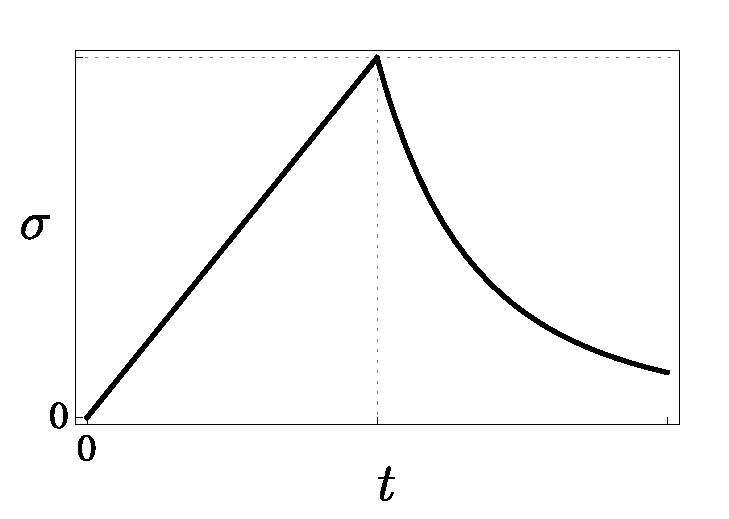
\includegraphics[width=0.45\textwidth]{at1hom}
          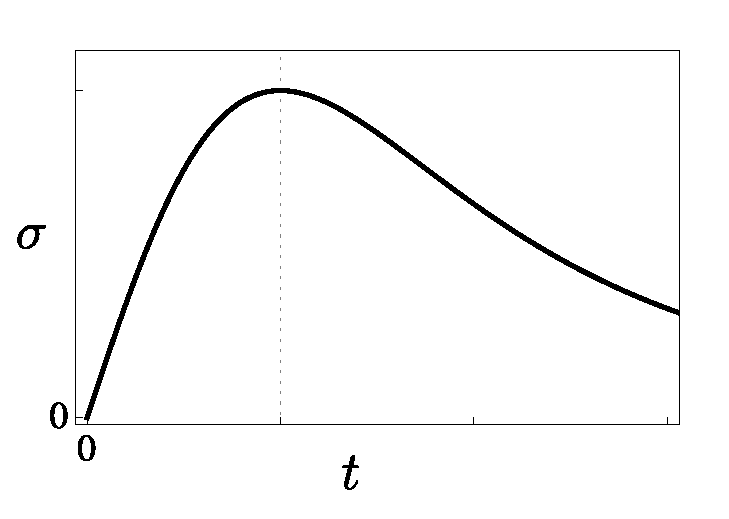
\includegraphics[width=0.45\textwidth]{at2hom}\\
      }
        %  \caption{Réponse en contrainte $\sigma$ en fonction du chargement $t$ monotone croissant pour les modèles $\mathsf{AT_1}$ et $\mathsf{AT_2}$.}
        %  \label{fig:response-homogene}
        %\end{figure}

        Indiquer à quel modèle correspond chaque courbe et identifier les zones à régime durcissant/adoucissant en contraintes. Que vaut la contrainte maximale $\sigma_M$ pour le modèle $\mathsf{AT_1}$ ?
     %Montrer que les réponses $\sigma-t$ sont cohérentes avec les réponses précédentes.
     % Marquer dans ces graphes les expressions de contraintes maximales $\sigma_M$, de la contrainte limite d'élasticité $\sigma_e$ et des valeurs correspondantes de $t$. Marquer les zones à régime durcissant/adoucissant en contraintes. 
     % \jb{Sans faire la question précédente, je mettrai plutôt.}
%\end{questions}

\section{Endommagement : solutions localisées}
On cherche à présent les solutions à endommagement non homogène. En particulier on cherche des solutions localisées dans une bande de largeur $D$ inconnue à l'intérieur du domaine.
$$
\begin{cases}
\alpha(x)>0, &x\in  (x_0-D/2,x_0+D/2),\\
\alpha(x)=0, & \text{autrement}
\end{cases}
$$
avec $x_0$ et $D$ tels que $0<x_0\pm D/2<L$.
Les solutions de ce type pour lesquels  $\max_x\alpha(x)=1$,  donc $\sigma=0$, sont assimilables à une approximation diffuse des fissures dans le modèle d'endommagement. 
On peut identifier la ténacité  effective du modèle d'endommagement, énergie dissipée pour la création d'une fissure, avec l'énergie dissipée dans ce type de solutions :
$$
\tilde G_c=w_1\int_{x_0-D/2}^{x_0+D/2}\left(w(\alpha(x))+\ell^2\left(\frac{d\alpha}{dx}\right)^2\right)\,dx
$$
\begin{comment}
\question \jb{Ne pas faire cette question ?} Montrer que les solutions doivent vérifier l'intégrale première suivante :
              $$
              \frac{E_0}{2w_1}(s(\alpha)-s(0))\,{\sigma^2}+w(\alpha)=\left(\frac{d\alpha}{dx}\right)^2\ell^2
              $$
            \begin{solution}
                On multiplie le critère en contraintes par $\alpha'(x)$ et on intègre entre $0$ et $L$ en tenant en compte que pour les solutions qu'on cherche soit $\alpha'(x)=0$ soit le critère est satisfait comme une égalité
            $$
                -
                \dfrac{\sigma^2}{2E_0}\frac{ds(\alpha)}{d\alpha}\frac{d\alpha}{dx}
                +
                \left(w'(\alpha)\frac{d\alpha}{dx} 
                -
                2 \ell^2\frac{d^2\alpha}{dx^2}\frac{d\alpha}{dx}\right)\,w_1
                =0
            $$
            donc
            $$
                -
                \dfrac{\sigma^2}{2E_0}s(\alpha)
                +
                \left(w(\alpha_i)
                -
                 \ell^2\left(\frac{d\alpha}{dx}\right)^2\right)\,w_1
                =c
            $$
            La valeur de la constante est déterminée en évaluant cette intégrale première dans la partie où $\alpha(x)=0$. On trouve $c=- \frac{\sigma^2}{2E_0}s(0)$.
            \end{solution}
\end{comment}
	\question \label{q:integrale-premiere} On cherche des solutions où la contrainte est nulle, avec $\sigma=
    0$ et
     $\alpha(x_0)=1$. %, voir Figure~\ref{atkhom}(droite). 
     Montrer que  $w(\alpha) -
                 \ell^2\left(\frac{d\alpha}{dx}\right)^2$ est une constante par rapport à $x$, puis que cette constante est nulle. En déduire que $\alpha'(x_0\pm D/2)=0$.
                 \begin{solution}
                 Le critère d'endommagement à contrainte nulle s'écrit:
                 $$
                 \left(w'(\alpha)
                -
                2 \ell^2\frac{d^2\alpha}{dx^2}\right)\,w_1
                =0
                 $$
                 où l'égalité au lieu de l'inégalité provient du fait qu'on cherche une solution où, soit $\alpha'(x)=0$ (en dehors de la zone de localisation), soit $\alpha'(x)>0$ dans la zone de localisation et donc on a égalité dans le critère. En multipliant par $\alpha'(x)$, on voit que:
                 $$ 
                 w'(\alpha)\frac{d\alpha}{dx}
                -
                2 \ell^2\frac{d^2\alpha}{dx^2}\frac{d\alpha}{dx} = \dfrac{d}{dx}\left(w(\alpha) -
                 \ell^2\left(\frac{d\alpha}{dx}\right)^2\right) = 0
                 $$
				Ainsi $w(\alpha) -
                 \ell^2\left(\frac{d\alpha}{dx}\right)^2$ est une constante. Celle-ci vaut 0 en évaluant l'expression dans la zone où $\alpha=0$. On a donc bien $\alpha'(x_0\pm D/2)=0$ en évaluant encore une fois cette expression en $x_0\pm D/2$.
                 \end{solution}
     \question Déterminer le profil d'endommagement respectant ces conditions pour le modèle $\mathsf{AT}_1$.
           \begin{solution}
            Le critère d'endommagement doit être vérifié comme une égalité dans la partie où l'endommagement est positif.
               Pour $\mathsf{AT}_1$
               $$
               \frac{d^2\alpha(x)}{dx^2}=\frac{1}{2\ell^2}
               $$
            En intégrant avec les conditions initiales $\alpha(x_0-D/2)=0$,
               $\alpha'(x_0-D/2)=0$, on trouve
               $$
               \alpha(x)=\frac{((x-x_0)-D/2))^2}{4\ell^2}
               $$
               En imposant $\alpha(x_0)=1$ on trouve
               $$
               D=4\ell
               $$
               On peut refaire le même raisonnement à partir de $x_0+D/2$. Le profil est symétrique par rapport à $x_0$.
               
           \end{solution}
    
 \question En utilisant le résultat de la question \ref{q:integrale-premiere}, montrer que 
 $$
 \tilde G_c=c_w{w_1\ell},\text{ avec }c_w=4\,\int_0^1\sqrt{w
 (\alpha)}d\alpha.
 $$
 et calculer $c_w$ pour les modèles $\mathsf{AT}_1$ et $\mathsf{AT}_2$.
 \begin{solution}
 On rappelle qu'on a montré que:
 $$
 w(\alpha)=\left(\frac{d\alpha}{dx}\right)^2\ell^2
 $$
 donc les deux termes dans $\tilde G_c$ donnent la même contribution 
 $$
\tilde G_c=w_1\int_{x_0-D/2}^{x_0+D/2}w(\alpha(x))+\ell^2\left(\frac{d\alpha}{dx}\right)^2\,dx=
2w_1\int_{x_0-D/2}^{x_0+D/2}\ell^2\left(\frac{d\alpha}{dx}\right)^2\,dx
$$
qu'on peut récrire avec un changement de variables :
$$\tilde G_c=
4w_1\ell\int_{\underbrace{x_0-D/2}_{\alpha=0}}^{\underbrace{0}_{\alpha=1}}\underbrace{\left(\ell\left(\frac{d\alpha}{dx}\right)\right)}_{\sqrt{w(\alpha)}}
\underbrace{\left(\frac{d\alpha}{dx}\right)\,dx}_{d\alpha}=
4w_1\int_{0}^{1}\ell^2\sqrt{w(\alpha)}\,d\alpha
$$
On calcule :
$$
c_w = 4 \int_0^1\sqrt{w(\alpha)}d\alpha  =
\begin{cases}
  \mathsf{AT_1}:& 8/3\\
  \mathsf{AT_2}:& 2\\
\end{cases}.
$$
 \end{solution}
    

	\question Donner la valeur de la constante $w_1$ à utiliser pour que
	      l'énergie dissipée dans ces solutions localisées avec $\sigma=0$ soit
	      équivalente à $G_c$, i.e.~à l'énergie dissipée dans une fissure dans le
	      modèle de rupture de Griffith.
          \begin{solution}
	      $$w_1=
          \begin{cases}
            \mathsf{AT_1}:& \frac{3G_c}{8\ell}\\
            \mathsf{AT_2}:& \frac{G_c}{2\ell}\\
          \end{cases}
          $$
          qui représente donc la densité locale d'énergie de dissipation du modèle d'endommagement local associé. On trouve donc que cette densité volumique varie en $G_c/\ell$ pour donner des solutions localisées 1D à énergie de dissipation indépendantes de $\ell$.
	      %et  que la limite d'élasticité de la barre est donnée par
	      %$$\sigma_c= \sqrt{\dfrac{3\,G_cE_0}{8\,\ell}}$$
          \end{solution}
	\question 
    Soit $\sigma_c$ la contrainte critique du matériau.
    Déterminer la valeur de la constante $\ell$ pour avoir $\sigma_M=\sigma_c$.  
    
    Étant donné les propriétés matérielles du béton : $E_0=30\,
    \mathrm{GPa}$, $G_c =50 \mathrm{N/m}$,  $\sigma_c = 4 \mathrm{MPa}$
    déterminer la valeur numérique de $\ell$ pour le modèle $\mathsf{AT_1}$. Que peut-on conclure quant à la taille caractéristique des structures que l'on peut modéliser avec un tel modèle ?
    \begin{solution}
        En identifiant $\sigma_c$ avec $\sigma_M$ on a
$$
    \begin{cases}
        \mathsf{AT_1}:&\sigma_M=\sqrt{2w_1 E_0}=\sqrt{\frac{3G_c E_0}{8\ell}}
        \Rightarrow
        \ell=\frac{3}{8}\frac{G_cE_0}{\sigma_c^2}
        \\
        \mathsf{AT_2}:& \sigma_M=2\sqrt{2w_1 E_0}=\sqrt{\frac{27G_c E_0}{256\ell}}=
        \frac{3\sqrt{3}}{16}\sqrt{\frac{G_c E_0}{\ell}}
        \Rightarrow
        \ell=\frac{27}{256}\frac{G_cE_0}{\sigma_c^2}
    \end{cases}
$$
Pour le béton on trouve  $\ell=3.5$cm pour $\mathsf{AT_1}$ et $1.0984922$cm $\mathsf{AT_2}$. On en déduit donc que l'utilisation de ces modèles pour le béton ne pourra conduire à des régularisation du modèle de Griffith que dans des situations où la taille caractéristique $L$ de la structure est très grande devant $\ell$. $L$ est donc typiquement de l'ordre du mètre, il n'est pas possible d'utiliser un tel modèle en conservant $\sigma_M=\sigma_c$ pour des échantillons de laboratoire de la taille du centimètre.
    \end{solution}

 %   \newline\underline{\textbf{Réponse 8:}}\vskip 5cm
    \end{questions}


\end{document}
